\chapter{Schwingungsvorgänge}
schwingfähiges System \\
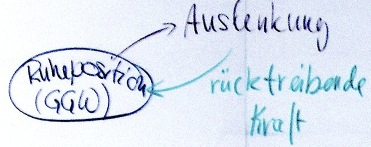
\includegraphics{Bild211}

\section{Energiebetrachtung}
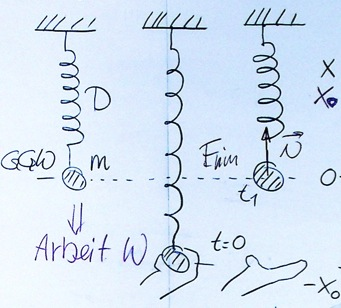
\includegraphics{Bild212} \\
\begin{itemize}
	\item gegeben durch Schwingsystem
	\item Anfangsbedingungen
\end{itemize}
harmonische Schwingung
\[ x(t) = \underbrace{x_0}_{\text{Amplitude}} \sin( \underbrace{\omega_0}_{\text{Kreisfrequenz}} t + \underbrace{\phi_0}_{\text{Phase}} ) \]
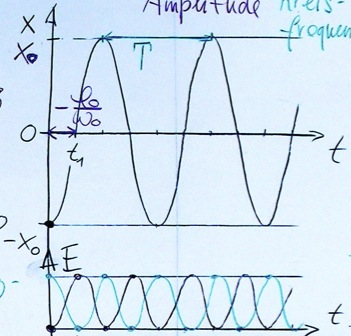
\includegraphics{Bild213}
\[
	E_{\text{tot}} = E_{\text{pot}} + E_{\text{kin}} = \text{ konst. } = W \\
	E_{\text{pot}} = \frac{1}{2} D x^2 \\
	E_{\text{kin}} = \frac{1}{2} m \dot{x}^2
\]
Kreisfrequenz $\omega_0$
\[ \text{(2.N.P.)} \quad \omega_o = \sqrt{\frac{D}{m}} \]
Schwingungsperiode $T$
\[ \boxed{ T = \frac{2\pi}{\omega_0} } \]
Frequenz $f = \frac{1}{T} = \frac{\omega_0}{2\pi}$

\begin{rep*}
	\uline{Das Induktionsgesetz} \\
	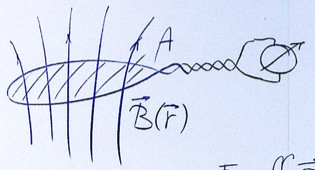
\includegraphics{Bild214} \\
	magn. Fluss
	\[ \Phi = \iint \vec{B} \cdot \vec{\dd A} \]
	Faraday's Induktionsgesetz
	\[ \boxed{ U_{\text{ind}} = -\frac{\dd \Phi}{\dd t} } \]
	
	\uline{Schwingungsvorgänge} \\
	\uline{harmonische Schwingung:}
	\[ \boxed{ x(t) = \underbrace*{x_0}_{\text{Amplitude}} \sin( \underbrace{\omega_0}_{\text{Kreisfrequenz}} t + \underbrace{\phi_0}_{\text{Phase}} ) } \]
	\begin{bsp*}[ note = Federpendel ]
		\[ \omega_0 = \sqrt{\frac{D}{m}} \]
	\end{bsp*}
	\uline{Energieerhaltung} \\
	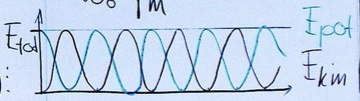
\includegraphics{Bild215}
	\[ E_{\text{tot}} = E_{\text{kin}}(t) + E_{\text{pot}}(t) = \frac{1}{2} m \dot{x}^2(t) + \frac{1}{2} D x^2(t) = W = \text{ konst.} \]
\end{rep*}

\section{Gedämpfte Schwingung}
Energie geht durch Reibung verloren! \\
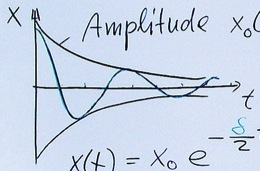
\includegraphics{Bild216}
\[
	\text{Amplitude } x_0(t) = x e^{-\frac{\delta}{2} t} \\
	x(t) = x_0 e^{-\frac{\delta}{2} t} \sin( \omega_d t + \phi_0 )
\]
schwache Dämpfung ($\delta$ klein) $\omega_d \approx \omega_0$
Energieverlust: $E_{\text{tot}} = E_{\text{pot}}( 0 ) \cdot e^{-\delta t}$

\section{Erzwungene Schwingung}
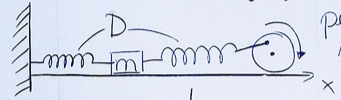
\includegraphics{Bild217} \\
periodische Anregung $F_0 \sin \omega t$ \\
2 Frequenzen!
\begin{itemize}
	\item ohne Anregung: $\omega_0 = \sqrt{\frac{D}{m}}$ Eigenfrequenz
	\item Anregungsfrequenz $\omega$ frei wählbar
\end{itemize}
Frage: Bewegung mit $\omega$ oder $\omega_0$? \\
Zu Beginn: Einschwingung mit $\omega_0$ (gedämpft) und $\omega$! \\
$t \rightarrow$ gross: stationärer Zustand. Nur noch $\omega$!

\subsection{Nur noch stationärer Zustand}
(mit Dämpfung: rasch im stationärem Zustand)
\[ \boxed{ x(t) = x_0(\omega) \cdot \sin( \omega t + \phi(\omega) ) } \]
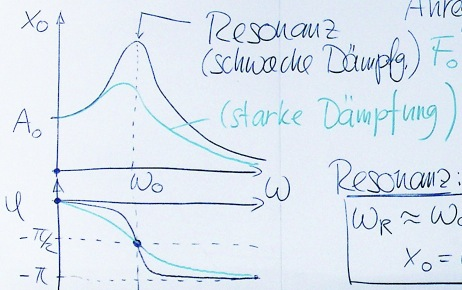
\includegraphics{Bild218} \\
Anregung: $F_0 \sin \omega t$ \\
Resonanz:
\[ \boxed{ \omega_R \approx \omega_0 , \phi = -\frac{\pi}{2} , x_0 = \text{ maximal} } \]

\subsection{Erklärung der Phase bei Resonanz}
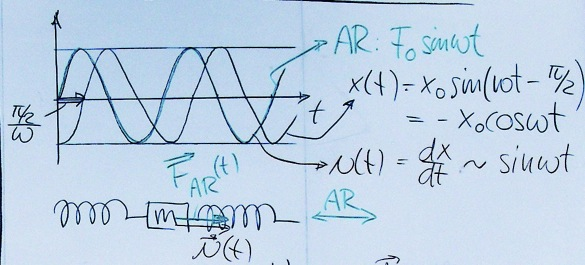
\includegraphics{Bild219}
\[ x(t) = x_0 \sin( \omega t - \frac{\pi}{2} = - x_0 \cos \omega t \]
$\implies$ Verschiebung $\vec{\dd r}$ \\
$\implies \vec{F_{AR}}$ verrichtet immer positive Arbeit!

\section{Anwendung: Magnetische Resonanztomographie (MRI)}
\subsection{Wasserstoffkern}
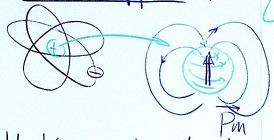
\includegraphics{Bild220} \\
\begin{itemize}
	\item Ladung $+e$
	\item Eigendrehimplus (Spin)
	\item magn. Moment $\vec{p_m}$
\end{itemize}
\subsection{\texorpdfstring{\ce{H}}{H}-Kerne in starkem Magnetfeld}
$\drsh$ magn. Moment $\vec{p_m}$ + Drehimpuls \\
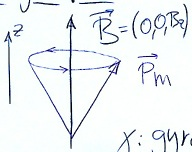
\includegraphics{Bild221} \\
$\implies$ Präzessionsbewegung \\
\[
	\vec{B} = ( 0 , 0 , B_z )
	\intertext{Präzessions-(Larmor-)Frequenz}
	\boxed{ \omega_L = \gamma \cdot B_z }
\]
$\gamma$: gyromagn. Verhältnis \\
Wasserstoffkern: $\gamma = 2\pi \cdot \SI{42.58}{\mega\hertz\per\tesla}$

\subsection{Kernresonanz-Spektroskopie}
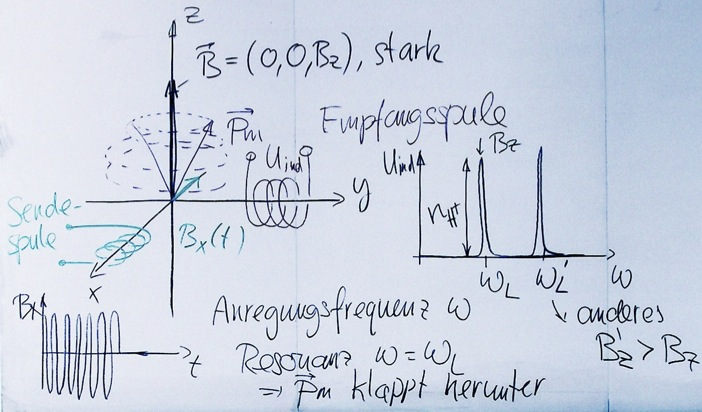
\includegraphics{Bild222} \\
Anregungsfrequenz $\omega$ \\
Resonanz $\omega = \omega_L$ \\
$\implies \vec{p_m}$ klappt herunter

\begin{rep*}[ note = Erzwungene Schwingung ]
	\uline{Anregung:} $F_0 \sin \omega t$ \\
	\uline{Schwingungssystem}, Eigenfrequenz $\omega_0$ \\
	$\implies$ stationärer Zustand:
	\[
		\boxed{ x(t) = x_0(\omega) \sin( \omega t + \phi(\omega) ) }
		\intertext{\uline{Resonanz:}}
		\boxed{ \begin{matrix*}[l]
			\omega_R \approx \omega_0 \\
			x_0( \omega_R ) \text{ maximal} \\
			\phi( \omega_R ) = -\frac{\pi}{2}
		\end{matrix*} }
	\]
	
	\uline{Kernresonanz-Spektroskopie (NMR)} \\
	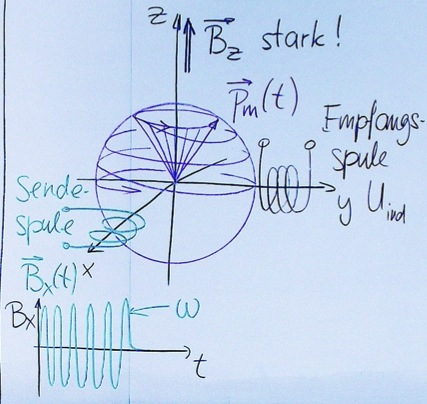
\includegraphics{Bild223} \\
	\uline{\ce{H}-Kerne}:
	\begin{itemize}
		\item Drehmpuls
		\item magn. Moment
	\end{itemize}
	$\implies$ Präzision mit
	\[ \boxed{ \omega_L = \gamma B_z } \]
	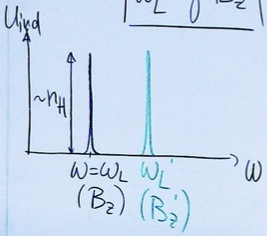
\includegraphics{Bild224}
\end{rep*}

\subsection{Gradientenfeld \texorpdfstring{$\vec{B_z}(\vec{r})$}{B\textsubscript{z}(r)}}
genau kennen!

\begin{itemize}[ label = $\implies$ ]
	\item Messe $U_{\text{ind}}$ bei $\omega_L( \vec{B_z} )$
	\item erhalte $U_{\text{ind}}( \vec{B_z}( \vec{r} ) )$
	\item $n_H( \vec{r} )$
\end{itemize}

\section{Wellen}
Was braucht es?
\begin{itemize}
	\item \uline{Medium}:
		\begin{bsp*}[ head = z.B. , note = Federkette ]
			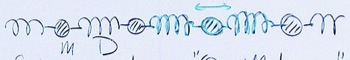
\includegraphics{Bild225}
		\end{bsp*}
		$\implies$ viele Schwingungssysteme, \enquote{\uline{Oszillatoren}} + Kopplung zwischen Oszillatoren \\
		Oszillatoren identisch $\implies$ resonante Ausbreitung
	\item \uline{Anregung} (=Welle): \enquote{Störung}, die sich im Medium ausbreitet \\
		$\implies$ Welle transportiert \uline{Energie}, nicht Masse!
\end{itemize}

\subsection{Polarisation}
= Bewegungsrichtung der einzelnen Oszillatoren \\
\uline{Pendel:} \\
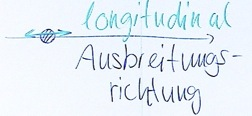
\includegraphics{Bild226} \\
Wellenmaschine: \\
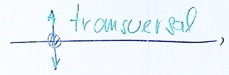
\includegraphics{Bild227}

\subsection{Ausbreitungsgeschwindigkeit \texorpdfstring{$c$}{c}}
\dots hängt ab von Medium (m,D)

\subsection{Mathematische Beschribung}
\[
	u( x , t ) = u( x - ct ) \quad ( \rightarrow \text{ pos. $x$-Richtg. } ) \\
	u( x , t ) = u( x + ct ) \quad ( \rightarrow \text{ neg. $x$-Richtg. } )
	\intertext{harmonische Wellen:}
	\begin{split}
		u( x , t )
			&= u_0 \sin( k ( x - ct ) ) \\
			&= u_0 \sin( \underbrace{k}_{\text{Wellenzahl } [ \si[ per-mode=reciprocal ]{\per\metre} ]} x - \underbrace{\omega}_{k \cdot c \\ \text{Kreisfreq.}} t ) \\
			&= u_0 \sin\left( \frac{2\pi}{\lambda} x - 2\pi \underbrace{f}_{\text{Frequenz}} \cdot t \right)
	\end{split}
\]

\subsection{Welle im Ortsbild}
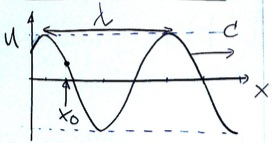
\includegraphics{Bild228} \\
Zeit $t_0$ fest
\[ u( x , t ) = u_0 \sin( kx - \underbrace{\omega t_0}_{\text{konst. Phase}} ) \]
Wellenlänge $\lambda$
\[ \boxed{ \lambda = \frac{2\pi}{k} } \]

\subsection{Welle im Zeitbild}
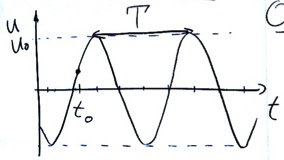
\includegraphics{Bild229} \\
\uline{Ort $x_0$ fest} (1 Oszillator!)
\[
	u( x_0 , t ) = u_0 \sin( \underbrace{k x_0}_{\text{konst. Phase}} - \omega t ) \\
	\boxed{ T = \frac{2\pi}{\omega} }
\]

\subsection{Wichtiger Zusammenhang}
\[ c = \frac{\lambda}{T} = \lambda \cdot f \]
\uline{Schallwellen} (Akustik) \\
\uline{Medium}: Luft, Wasser, FK \\
\uline{Anregung} $u( x , t )$: longitudinale Auslenkung von Luftschichten \\
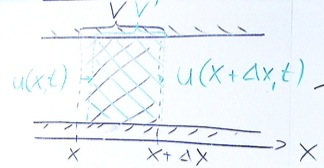
\includegraphics{Bild230}
\[ u( x , t ) = u_0 \sin( kx - \omega t ) \]
hier: $V' < V$ \\
Luft komprimiert!
\begin{def*}[ note = Schalldruck , index = Schalldruck ]
	\[ p_s( x , t ) = p( x , t ) - p_0 = - \underbrace{p_s^0}_{\text{Schalldruckamplitude}} \cos( kx - \omega t ) \]
\end{def*}

\uline{Ortsbild}: \\
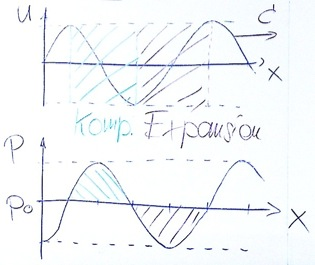
\includegraphics{Bild231} \\
Schallgeschwindigkeit $c$ \\
\uline{Luft}:
\[ c = \sqrt{\frac{RT \kappa}{M}} = \sqrt{\frac{\frac{7}{5} p_0}{\rho}} \approx \SI{350}{\metre\per\second} \]

\subsection{Intensität}
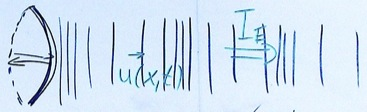
\includegraphics{Bild232} \\
Energiestrom $I_E$ ( $\si{\joule\per\second} = \omega$ )
\[
	I_E = \underbrace*{\frac{1}{2} \rho}_{\text{kin. Energie pro Vol.}} \underbrace*{v_0^2}_{\text{\enquote{Schallschnelle}}} \cdot A \cdot c \\
	u( x , t ) \quad x = x_0 \\
	\implies v( x , t ) = \frac{\dd u( x , t ) }{\dd t} \\
	\text{Amplitude } v_0
	\intertext{\uline{Intensität}:}
	I = \frac{I_E}{A} = \frac{1}{2} \rho v_0^2 \cdot c = \frac{1}{2} \rho \omega^2 u_0^2 c \\
	\begin{bmatrix}
		u( x , t ) = u_0 \sin( kx - \omega t ) \\
		\implies v_0 = \omega \cdot u_0
	\end{bmatrix} \quad \dots \quad \boxed{ I = \frac{(p_s^0)^2}{2 \cdot \rho \cdot c} } \\
	\boxed{ I \sim u_0^2 }
\]

\subsection{Menschliches Ohr}
Hörschwelle $I_0 = 10^{-12}\si{\watt\per\metre\squared}$ \\
Schmerzgrenze $I_S \approx \SI{1}{\watt\per\metre\squared}$ \\
$\implies$ Wahrnehmung logarithmisch!

\subsubsection{Schallpegel}
\[ \boxed{ L = 10 \cdot \log_{10} \frac{I}{I_0} } \text{ in dezibel } \si{\deci\bel} \]
\begin{bsp*}
	\[
		I = I_0 \implies L = 0 \\
		\text{Schalldruckampl. } p_s^0 = \sqrt{2 \rho c I} = \SI{2e-5}{\pascal} = \SI{2e-10}{\bar}
	\]
\end{bsp*}

\begin{rep*}[ note = Harmonische Wellen ]
	\[ u( x , t ) = u_0 \sin( kx - \omega t ) \]
	$t = t_0$: 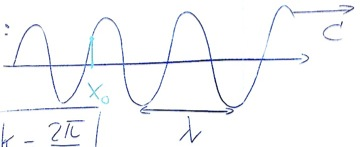
\includegraphics{Bild233} \\
	\[
		\boxed{ k = \frac{2\pi}{\lambda} } \\
		\boxed{ \omega = 2 \pi f = \frac{2\pi}{T} } \\
		\boxed{ c = \frac{\lambda}{T} }
	\]
	
	\uline{Schallwellen} (in Gasen) \\
	$u( x , t )$: longitudinale Auslenkung von Luftschichten \\
	$p_s( x , t )$: \uline{Schalldruck} \\
	\uline{Schallgeschwindigkeit}
	\[ c = \sqrt{\frac{\frac{7}{5} p_0}{\rho}} \approx \SI{350}{\metre\per\second} \]
	\uline{Intensität}:
	\[ I = \frac{1}{2} \rho \omega^2 u_0^2 c = \frac{(p_s^0)^2}{2 \rho c} \]
	\uline{Schallpegel}:
	\[ \boxed{ L = 10 \cdot \log_{10} \frac{I}{I_0} } \text{ in \si{\deci\bel};  mit } I_0 = 10^{-12} \si{\watt\per\metre\squared} \]
	\begin{bsp*}[ head = z.B. ]
		\[
			L = \SI{80}{\deci\bel} \\
			80 = 10 \log \frac{I}{I_0} \implies 10^8 = \frac{I}{ 10^{-12} \si{\watt\per\metre\squared} }
		\]
	\end{bsp*}
\end{rep*}

\subsection{Hören von Schallwellen}
\begin{itemize}
	\item \uline{reiner Ton}: genau 1 Frequenz $f = \frac{\omega}{2\pi}$
		\[ \implies u( x , t ) = u_0 \sin( kx - \omega t ) \]
		Mittelohr: $x = x_0 = 0$ \\
		$\implies u_0 \sin \omega t \implies$ Frequenz $\rightcurvedarrow$ Ort der Anregung auf Kochlea
	\item \uline{Zwei Frequenzen}
		\[ u(t) = u_0 \sin\left( \frac{\omega_1 + \omega_2}{2} \right ) t \cdot \cos\left( \frac{\omega_1 - \omega_2}{2} \right) \]
		\uline{2 Fälle:}
		\begin{itemize}
			\item $\omega_1 , \omega_2$ stark verschieden \\
				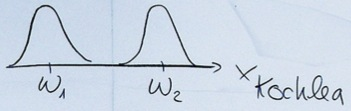
\includegraphics{Bild234}
			\item $\omega_1 \approx \omega_2$ \\
				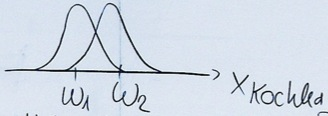
\includegraphics{Bild235}
				\[ \left. \begin{matrix*}[l]
					\implies \text{ mittlerre Frequenz } \frac{\omega_1 + \omega_2}{2} \\
					\implies \text{ Amplitude } 2 u_0 \cos\left( \frac{\omega_1 - \omega_2}{2} \right) t
					\end{matrix*} \right\} \quad \text{Schwebung}
				\]
		\end{itemize}
	\item \uline{Klang}: $u(t)$ ist periodische Funktion \\
		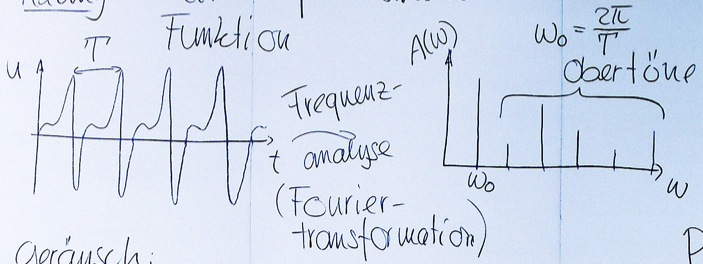
\includegraphics{Bild236}
	\item \uline{Geräusch}: $u(t)$ nicht periodisch \\
		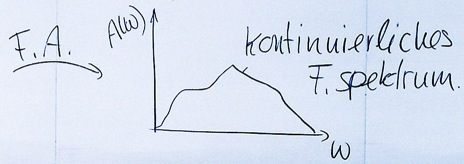
\includegraphics{Bild237} \\
		\uline{Pistolenknall}: \\
		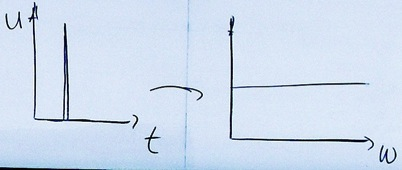
\includegraphics{Bild238}
\end{itemize}

\subsection{Ultraschall}
( $f \approx \SI{20}{\kilo\hertz} - \SI{100}{\mega\hertz}$ )

\subsubsection{Reflexion und Transmission}
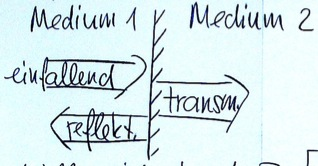
\includegraphics{Bild239} \\
$M_1$: Luft \\
$M_2$: Wasser \\
\uline{Wellenwiderstand} $Z_W$
\[ \boxed{ Z_W = \rho \cdot c } \]
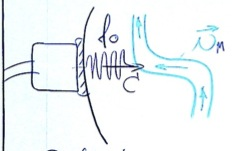
\includegraphics{Bild240} \\
Reflexion an inhomogenitäten im Blut ( $\implies$ bewegtes Medium ) \\
Erregung des Mediums (Blut)
\[ f' = f_0 \left( 1 + \frac{v_M}{c} \right) \]
(D.E. bei bewegtem Empfänger) \\
Erzeugt reflektierte Welle
\[ f^R = \frac{f'}{\left( 1 - \frac{v_M}{c} \right) } \]
(D.E. bei bewegtem Sender) \\
$\implies f^R \approx f_0 \left( 1 + 2 \frac{v_M}{c} \right)$ \\
$\implies$ 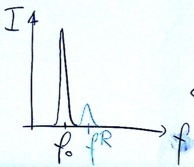
\includegraphics{Bild241}
